En esta sección se detallan los resultados obtenidos en el conjunto de prueba, el cual representa el 15\% de las muestras del conjunto de datos detallado en el capítulo 3, para esta tarea se seleccionaron los tres mejores modelos entrenados según la métrica de precisión global en el conjunto de validación. Además, como parte de una evaluación adicional, se emplearon los datos restantes del conjunto de datos recolectado junto con el conjunto de datos “offendes" para formar un nuevo conjunto de datos. Este nuevo conjunto se evaluó con cada uno de los modelos seleccionados. Finalmente se presentaran más métricas de evaluación sobre el conjunto de prueba y el mejor modelo de red neuronal convolucional.

\begin{itemize}
\item Nuevo conjunto de prueba
\end{itemize}
Se creó un nuevo conjunto de datos utilizando las muestras restantes del conjunto total recolectado que no fueron utilizadas en el proceso de entrenamiento, validación y prueba de los modelos. Es importante destacar que la única categoría con datos extraídos exclusivamente de redes sociales bolivianas es la de ``lenguaje no ofensivo''. La categoría de ``lenguaje ofensivo'' es una combinación de datos extraídos tanto de redes sociales bolivianas como del conjunto de datos ``offendes''. Por otro lado, la categoría ``grosero'' está compuesta totalmente por datos generados por el modelo de lenguaje ChatGPT, es decir, son datos completamente nuevos.

El número de muestras utilizadas del conjunto de datos extraído de redes sociales bolivianas se denomina ``conjunto recolectado'', mientras que el número de muestras del conjunto ``offendes'' se denomina ``conjunto Offendes''. Este conjunto de datos se utilizó inicialmente para el etiquetado de datos, dado que aunque fueron recolectados en un contexto cultural diferente el tema principal era útil para esta tarea.

Los detalles específicos de este nuevo conjunto de datos se encuentran detallados en la tabla \ref{tbl:categorias}.

\begin{table}[!ht]
	\centering
	\begin{tabular}{|c|c|c|c|c|}
		\hline
		\textbf{Categorías} & \textbf{Conjunto recolectado} & \textbf{Conjunto Offendes} & \textbf{Conjunto generado} & \textbf{Total} \\ \hline
		Ofensivos & 799 & 4201 & 0 & 5000 \\ \hline
		No ofensivos & 5000 & 0 & 0 & 5000 \\ \hline
		Groseros & 0 & 0 & 182 & 182 \\ \hline
		\textbf{Total} & 5799 & 4201 & 182 & 10182 \\ \hline
	\end{tabular}
	\caption{Distribución de categorías en el nuevo conjunto de datos}
	\label{tbl:categorias}
\end{table}

\begin{itemize}
\item Desempeño con los conjuntos de prueba
\end{itemize}

A continuación se presentan los resultados obtenidos por los tres modelos seleccionados tanto en el conjunto de prueba original como en el conjunto de prueba nuevo. Estos resultados se detallan en la tabla \ref{tbl:resultados}, permitiendo así evaluar la capacidad de generalización de cada modelo.


\begin{table}[!ht]
	\centering
	\begin{tabular}{|c|c|c|c|c|}
		\hline
		~ & \multicolumn{2}{|c|}{\textbf{Conjunto de prueba}} & \multicolumn{2}{|c|}{\textbf{Conjunto nuevo}} \\ \hline
		\textbf{Nombre del modelo} & \textbf{Precisión} & \textbf{Pérdida} & \textbf{Precisión} & \textbf{Pérdida} \\ \hline
		cnn\_base\_bndp\_32t & 0.7931 & 0.5348 & 0.5136 & 1.4332 \\ \hline
		cnn\_two & 0.7726 & 0.5524 & 0.5023 & 1.2967 \\ \hline
		cnn\_dp\_two & 0.7937 & 0.5205 & 0.5018 & 1.2430 \\ \hline
	\end{tabular}
	\caption{Resultados de los modelos en diferentes conjuntos}
	\label{tbl:resultados}
\end{table}


En los resultados detallados en la tabla \ref{tbl:resultados}, se observa lo siguiente:

\begin{itemize}

\item El modelo cnn\_dp\_two demostró tener la mayor capacidad de generalización en el conjunto de datos de prueba bajo el contexto boliviano. Ya que alcanzó la menor pérdida y la mayor precisión en comparación con los otros dos modelos.

\item En el conjunto de datos nuevo, que incluye principalmente las muestras recolectadas en contextos no bolivianos del conjunto de datos “offendes”, el modelo cnn\_base\_bndp\_32t exhibió la mejor capacidad de generalización, aunque sus resultados no difieren significativamente de los otros modelos. Para este conjunto de datos se observa una disminución en la precisión y un aumento en la pérdida, este fenómeno es completamente normal debido a las diferencias culturales y contextuales entre los conjuntos de datos.

\end{itemize}

Es relevante destacar que la pérdida en el conjunto de datos de prueba bajo el contexto boliviano siempre se mantiene por debajo del 60\%. Además, la precisión de todos los modelos en este conjunto de datos siempre supera el 70\%.

\begin{itemize}
\item Evaluación del mejor modelo
\end{itemize}

A continuación se presentan los resultados de las métricas de precisión, sensibilidad y puntaje F1 del modelo cnn\_dp\_two para cada una de sus clases en el conjunto de datos de prueba bajo el contexto boliviano. Los detalles se encuentran en la tabla \ref{tbl:metrics}.

\begin{table}[!ht]
	\centering
	\begin{tabular}{|c|c|c|c|}
		\hline
		\textbf{Clase} & \textbf{Precisión} & \textbf{Sensibilidad} & \textbf{F1-Score} \\ \hline
		0 & 0.8269 & 0.8060 & 0.8163 \\ \hline
		1 & 0.7562 & 0.8181 & 0.7858 \\ \hline
		2 & 0.9082 & 0.3938 & 0.5480 \\ \hline
	\end{tabular}
	\caption{Métricas de rendimiento por clase}
	\label{tbl:metrics}
\end{table}


Los resultados de la matriz de confusión para el modelo cnn\_dp\_two1 se pueden consultar en la Imagen \ref{fig:matriz}.


\begin{figure}[!h]
	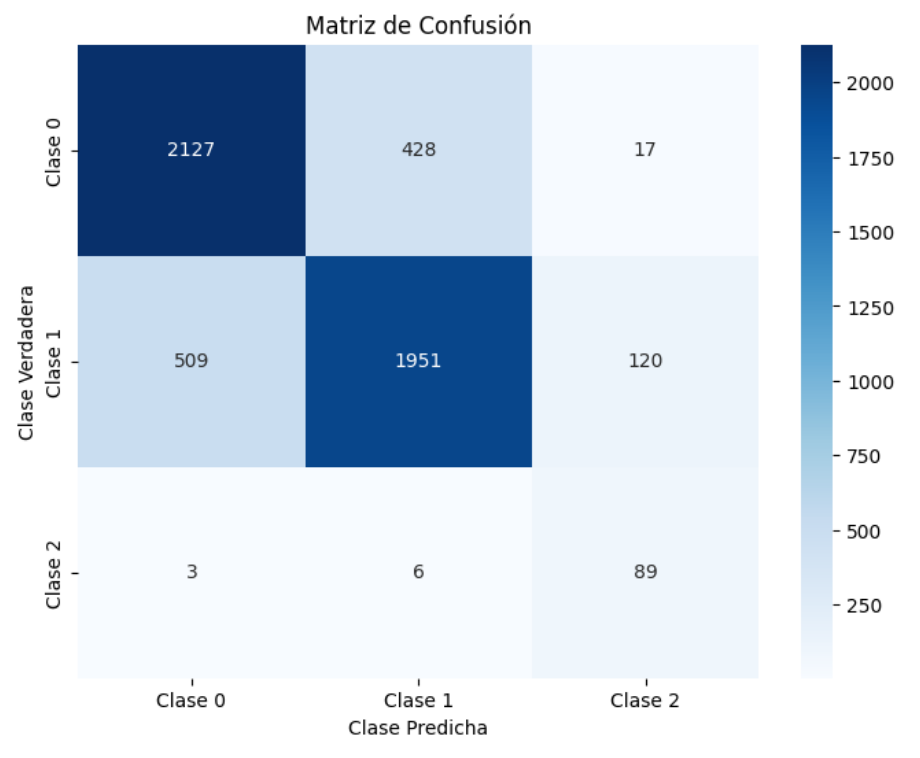
\includegraphics[width=0.8\textwidth]{capitulo5/figuras/matriz_confusion.PNG}
	\caption{Matriz de Confusión }
	\floatfoot{Fuente: Elaboración propia}
	\label{fig:matriz}
\end{figure}

Los resultados de la matriz se pueden interpretar como:

\begin{itemize}

\item Clase 0:
Verdaderos Positivos (TP) = 2127
Falsos Negativos  (FN) = 428 + 17 = 445 (Ejemplos de clase 0 clasificados como 1 o 2)
Falsos Negativos Positivos (FP) = 509 + 3 = 512 (Ejemplos de clase 1 o 2 clasificados como 0)


\item Clase 1:
Verdaderos Positivos (TP) = 1951
Falsos Negativos (FN) = 509 + 120 = 629 (Ejemplos de clase 1 clasificados como 0 o 2)
Falsos Positivos (FP) = 428 + 6 = 434 (Ejemplos de clase 0 o 2 clasificados como 1)

\item Clase 2:
Verdaderos Positivos (TP) = 89
Falsos Negativos (FN) = 3 + 6 = 9 (Ejemplos de clase 2 clasificados como 0 o 1)
Falsos Positivos (FP) = 17 + 120 = 137 (Ejemplos de clase 0 o 1 clasificados como 2)

\end{itemize}

\textbf{Análisis de las métricas de evaluación}

El análisis del desempeño del modelo cnn\_dp\_two revela los siguientes puntos importantes:

\begin{itemize}

\item Desempeño Desbalanceado:
El modelo muestra un buen desempeño en las Clases 0 y 1, con recall y precisión relativamente altos. 

\item Alta Precisión en Clase 2:
La Clase 2 muestra una alta precisión (aproximadamente 0.908), lo que indica que cuando el modelo predice la Clase 2, generalmente es correcto. Sin embargo, el bajo recall sugiere que no está detectando suficientes instancias de la Clase 2.

\item Falsos Positivos y Negativos:
Para la Clase 0 y la Clase 1, hay un número considerable de falsos positivos y falsos negativos. Esto sugiere que el modelo está confundiendo estas clases entre sí.


\end{itemize}

